\documentclass[a4paper, 10pt, twoside]{article}
\usepackage[left=2cm, right=2cm, top=2cm, bottom=3cm]{geometry}
\usepackage{amsmath}
\usepackage[shortlabels]{enumitem}
\usepackage{cases}
\usepackage{systeme}
\usepackage{graphicx}
\usepackage[hidelinks]{hyperref}
\usepackage{commath}

\begin{document}

\title{Machine Learning - Theoretical exercise 2}
\author{T\'eo Bouvard}
\maketitle

\section*{Problem 1}
\begin{enumerate}[a)]
    \item In the following, we use the notation $\lambda(\alpha_i \mid \omega_j) \Leftrightarrow \lambda_{ij}$
          \begin{align*}
              \lambda_{11} & = 0    & \text{correct classification of toxic container}       \\
              \lambda_{21} & = 10^5 & \text{incorrect classification of toxic container}     \\
              \lambda_{22} & = 0    & \text{correct classification of non-toxic container}   \\
              \lambda_{12} & = 250  & \text{incorrect classification of non-toxic container} \\
          \end{align*}

    \item
          \begin{align*}
              R(\alpha_1 \mid x) & = \lambda_{11}P(\omega_1 \mid x) + \lambda_{12}P(\omega_2 \mid x) \\
              R(\alpha_2 \mid x) & = \lambda_{21}P(\omega_1 \mid x) + \lambda_{22}P(\omega_2 \mid x) \\
          \end{align*}
          As $\lambda_{11} = 0$ and $\lambda_{22} = 0$,
          \begin{align*}
              R(\alpha_1 \mid x) & = \lambda_{12}P(\omega_2 \mid x) \\
              R(\alpha_2 \mid x) & = \lambda_{21}P(\omega_1 \mid x) \\
          \end{align*}\label{eq:risk}

    \item To determine the decision boundary that minimizes the average cost, we solve the equality of conditional loss functions.
          \begin{align*}
              R(\alpha_1 \mid x)                                                          & = R(\alpha_2 \mid x)                                                  \\
              \lambda_{12}P(\omega_2 \mid x)                                              & = \lambda_{21}P(\omega_1 \mid x)                                      \\
              \frac{\lambda_{12}}{\lambda_{21}}\frac{P(\omega_2)P(x \mid \omega_2)}{P(x)} & = \frac{P(\omega_1)P(x \mid \omega_1)}{P(x)} & \text{(Bayes Theorem)} \\
              \frac{\lambda_{12}P(\omega_2)}{\lambda_{21}P(\omega_1)}P(x \mid \omega_2)   & = P(x \mid \omega_1)                                                  \\
          \end{align*}
          Let $K = \frac{\lambda_{12}P(\omega_2)}{\lambda_{21}P(\omega_1)}$. Furthermore, we know that $P(x \mid \omega_1) \sim \mathcal{N}(\mu_1,\sigma^{2})$ and $P(x \mid \omega_2) \sim \mathcal{N}(\mu_2,\sigma^{2})$.
          \begin{align*}
              K\frac{1}{\sigma\sqrt{2\pi}}e^{-\frac{(x-\mu_1)^2}{2\sigma^2}}            & = \frac{1}{\sigma\sqrt{2\pi}}e^{-\frac{(x-\mu_2)^2}{2\sigma^2}} \\
              \ln{(Ke^{-\frac{(x-\mu_1)^2}{2\sigma^2}})}                                & = \ln{(e^{-\frac{(x-\mu_2)^2}{2\sigma^2}})}                     \\
              \ln K - \frac{(x-\mu_1)^2}{2\sigma^2}                                     & = -\frac{(x-\mu_2)^2}{2\sigma^2}                                \\
              \ln K + \frac{1}{2\sigma^2}((x-\mu_2)^2 - (x-\mu_1)^2)                    & = 0                                                             \\
              \ln K + \frac{1}{2\sigma^2}(x^2 -2\mu_2x+\mu_2^2-x^2+2\mu_1x-\mu_1^2)     & = 0                                                             \\
              \ln K + \frac{1}{2\sigma^2}(2x(\mu_1-\mu_2)+\mu_2^2-\mu_1^2)              & = 0                                                             \\
              \ln K + \frac{\mu_1-\mu_2}{\sigma^2}x + \frac{\mu_2^2-\mu_1^2}{2\sigma^2} & = 0                                                             \\
              \frac{\mu_1-\mu_2}{\sigma^2}x                                             & = \frac{\mu_1^2-\mu_2^2}{2\sigma^2} - \ln K                     \\
              x                                                                         & = \frac{\mu_1^2-\mu_2^2}{2(\mu_1-\mu_2)} - \sigma^2\ln K        \\
              x                                                                         & = \frac{\mu_1 + \mu_2}{2} - \frac{\sigma^2}{\mu_1-\mu_2}\ln K   \\
          \end{align*}
          Numerically solving this equation gives us the decision boundary (CHECK STRANGE RESULT?)
          \begin{align*}
              x_{lim} & = \frac{0.4 + 0.2}{2} - \frac{10^{-4}}{0.4-0.2} \times \ln (\frac{25\times250}{10^5}) \\
              x_{lim} & = 0.3014
          \end{align*}
    \item To determine the minimum average cost $R_{min}$ upon classification, we can use either of the two equations derived in question \ref{eq:risk}.
          \begin{align*}
              R_{min} & = \lambda_{12}P(\omega_2 \mid x_{lim})                                                                                              \\
                      & = \lambda_{12}\frac{P(\omega_2)P(x_{lim} \mid \omega_2)}{P(x_{lim})}                                                                \\
                      & = \lambda_{12}\frac{P(\omega_2)P(x_{lim} \mid \omega_2)}{P(\omega_1)P(x_{lim} \mid \omega_1) + P(\omega_2)P(x_{lim} \mid \omega_2)} \\
                      & = \lambda_{12}\frac{1}{\frac{P(\omega_1)}{P(\omega_2)}\frac{P(x_{lim} \mid \omega_1)}{P(x_{lim} \mid \omega_2)} + 1}                \\
          \end{align*}
          We are given $\frac{P(\omega_1)}{P(\omega_2)} = \frac{1}{25}$, we need to compute $\frac{P(x_{lim} \mid \omega_1)}{P(x_{lim} \mid \omega_2)}$

          \begin{align*}
              \frac{P(x_{lim} \mid \omega_1)}{P(x_{lim} \mid \omega_2)} & = \frac{\frac{1}{\sigma\sqrt{2\pi}}e^{-\frac{(x_{lim}-\mu_1)^2}{2\sigma^2}}}{\frac{1}{\sigma\sqrt{2\pi}}e^{-\frac{(x_{lim}-\mu_2)^2}{2\sigma^2}}} \\
                                                                        & = e^{{\frac{(x_{lim}-\mu_2)^2-(x_{lim}-\mu_1)^2}{2\sigma^2}}}
          \end{align*}

          So
          \begin{align*}
              R_{min} & = 249.4 \text{ NOK}
          \end{align*}

          OR P(error) with integral ?
          \begin{align*}
              R_{min} & = P(w_2)P(x < x_{lim} \mid w_2) + P(w_1)P(x > x_{lim} \mid w_1)                                       \\
              R_{min} & = P(w_2) \int_{-\infty}^{x_{lim}} P(x \mid w_2) dx + P(w_1) \int_{x_{lim}}^{+\infty} P(x \mid w_1) dx
          \end{align*}
          To get $P(w_1) \text{ and } P(w_2)$, we use the fact that
          \begin{align*}
              \begin{cases}
                  P(w_1)+P(w_2)         & = 1  \\
                  \frac{P(w_2)}{P(w_1)} & = 25
              \end{cases}
              \implies
              \begin{cases}
                  P(w_1) & = \frac{1}{26}  \\
                  P(w_2) & = \frac{25}{26}
              \end{cases}
          \end{align*}
          Furthermore,
          \begin{align*}
              \int_{-\infty}^{x_{lim}} P(x \mid w_2) dx & = P(u < \frac{x_{lim} - \mu_1}{\sigma}) \\
                                                        & = ?
          \end{align*}
\end{enumerate}

\section*{Problem 2}
\begin{enumerate}[a)]
    \item
          \begin{align*}
              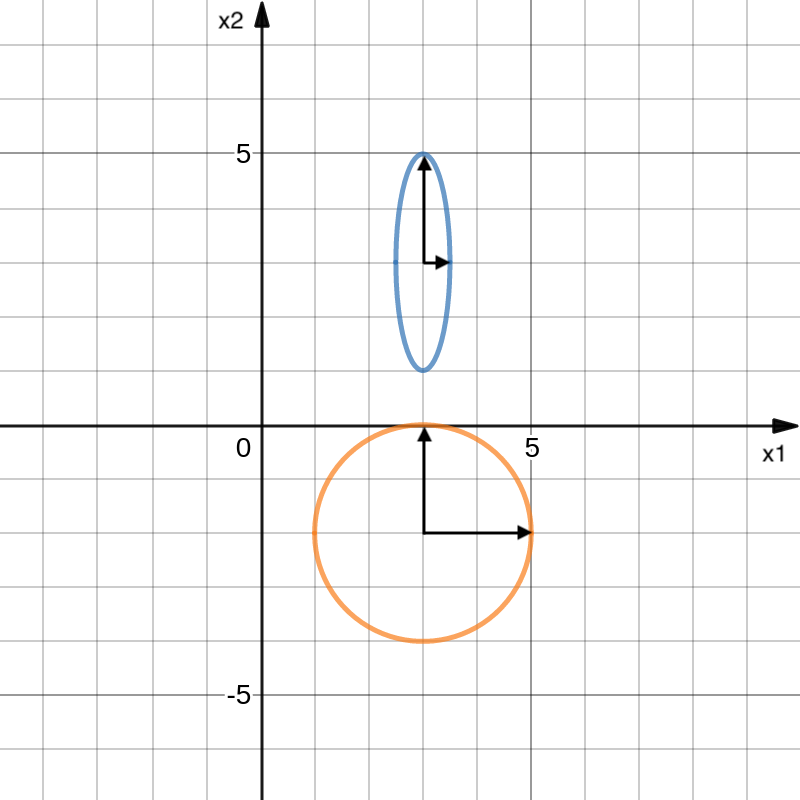
\includegraphics[width=0.5 \textwidth]{contour.png}
          \end{align*}
    \item
          The risk function $g$ can be defined as $g_i(x) = \ln P(\omega_i) + \ln P(x \mid \omega_i)$ for $i = 1, 2$. In this exercise, priors are equal so they can be omitted when solving the equality of risk for both classes.
          \begin{align*}
              g_1(x)                                   & = g_2(x)                                   \\
              \ln P(\omega_1) + \ln P(x \mid \omega_1) & = \ln P(\omega_2) + \ln P(x \mid \omega_2) \\
              \ln P(x \mid \omega_1)                   & = \ln P(x \mid \omega_2)                   \\
          \end{align*}
          Furthermore, the feature vectors of the two classes are normally distributed, meaning that
          \begin{align*}
              P(x \mid \omega_i) = \frac{1}{(2\pi)^{\frac{d}{2}} \begin{vmatrix}\Sigma_i\end{vmatrix}^{\frac{1}{2}}} e^{-\frac{1}{2}(x-\mu_i)^T \Sigma_i^{-1}(x-\mu_i)} &  & i = 1, 2 \\
          \end{align*}
          So the previous equality becomes
          \begin{align*}
              -\frac{d}{2} \ln 2\pi - \frac{1}{2} \ln \begin{vmatrix}\Sigma_1\end{vmatrix} - \frac{1}{2}(x-\mu_1)^T \Sigma_1^{-1}(x-\mu_1) & = -\frac{d}{2} \ln 2\pi - \frac{1}{2} \ln \begin{vmatrix}\Sigma_2\end{vmatrix} - \frac{1}{2}(x-\mu_2)^T \Sigma_2^{-1}(x-\mu_2) \\
              - \frac{1}{2} \ln \begin{vmatrix}\Sigma_1\end{vmatrix} - \frac{1}{2}(x-\mu_1)^T \Sigma_1^{-1}(x-\mu_1)                       & = - \frac{1}{2} \ln \begin{vmatrix}\Sigma_2\end{vmatrix} - \frac{1}{2}(x-\mu_2)^T \Sigma_2^{-1}(x-\mu_2)                       \\
          \end{align*}
          The covariance matrices $\Sigma_i$ have nice properties allowing us to simplify this equation.
          \begin{align}
              \begin{vmatrix}\Sigma_1\end{vmatrix} = \begin{vmatrix}\frac{1}{2} & 0 \\ 0 & 2\end{vmatrix} = 1 \implies \frac{1}{2} \ln \begin{vmatrix}\Sigma_1\end{vmatrix} = 0            \\
              \begin{vmatrix}\Sigma_2\end{vmatrix} = \begin{vmatrix}2 & 0 \\ 0 & 2\end{vmatrix} = 4 \implies \frac{1}{2} \ln \begin{vmatrix}\Sigma_2\end{vmatrix} = \ln 2        \\
              \Sigma_1^{-1} = \begin{bmatrix}\frac{1}{2} & 0 \\ 0 & 2\end{bmatrix}^{-1} = \begin{bmatrix}2 & 0 \\ 0 & \frac{1}{2}\end{bmatrix} &  & \text{because } \Sigma_1 \text{ is diagonal} \\
              \Sigma_2^{-1} = \begin{bmatrix}2 & 0 \\ 0 & 2\end{bmatrix}^{-1} = \begin{bmatrix}\frac{1}{2} & 0 \\ 0 & \frac{1}{2}\end{bmatrix} &  & \text{because } \Sigma_2 \text{ is diagonal}
          \end{align}
          This allows us to write the previous equality as
          \begin{align*}
              - \frac{1}{2}(x-\mu_1)^T \Sigma_1^{-1}(x-\mu_1) + \frac{1}{2}(x-\mu_2)^T \Sigma_2^{-1}(x-\mu_2)  + \ln 2                                                                                              & = 0   \\
              - \frac{1}{4}\begin{bmatrix}x_1-3 \\ x_2-3\end{bmatrix}^T \begin{bmatrix}4 & 0 \\ 0 & 1\end{bmatrix}\begin{bmatrix}x_1-3 \\ x_2-3\end{bmatrix} + \frac{1}{4}\begin{bmatrix}x_1-3 \\ x_2+2\end{bmatrix}^T\begin{bmatrix}1 & 0 \\ 0 & 1\end{bmatrix}\begin{bmatrix}x_1-3 \\ x_2+2\end{bmatrix}  + \ln 2 & = 0   \\
              - \frac{1}{4}[(4x_1-12)(x_1-3)+(x_2-3)^2] + \frac{1}{4}[(x_1-3)^2+(x_2+2)^2] + \ln 2                                                                                                                  & = 0   \\
              -\frac{1}{4}(4x_1^2 -24x_1 + 36 + x_2^2 -6x_2+9) + \frac{1}{4}(x_1^2-6x_1+9+x_2^2+4x_2+4) + \ln 2                                                                                                     & = 0   \\
              \frac{3}{4}x_1^2 + \frac{9}{2}x_1 -8 + \ln 2                                                                                                                                                          & = x_2
          \end{align*}
          Thus, the decision border is a parabola.
    \item
          \begin{align*}
              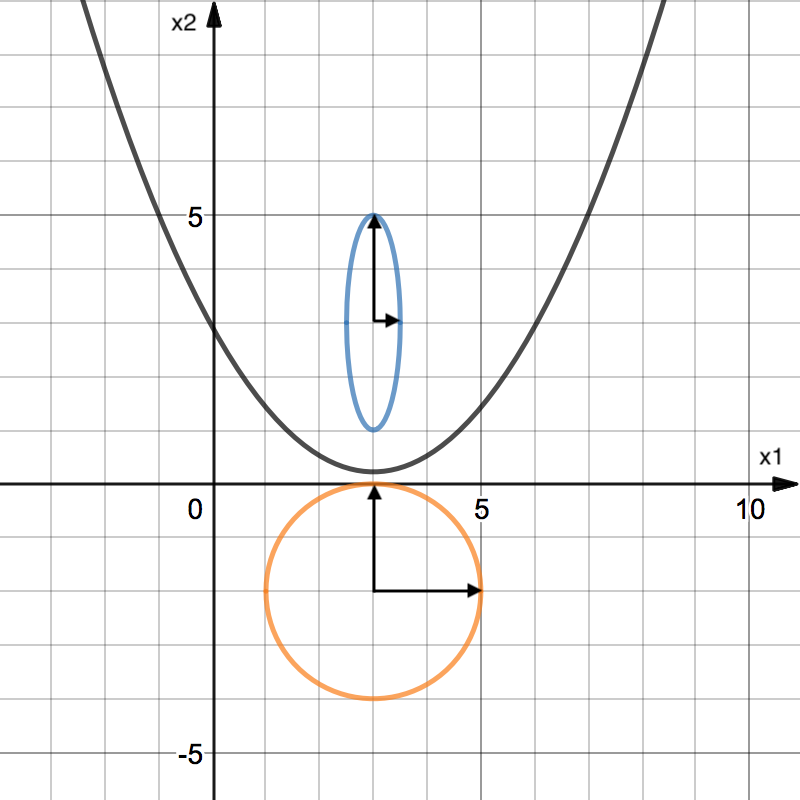
\includegraphics[width=0.5 \textwidth]{border.png}
          \end{align*}
\end{enumerate}

\section*{Problem 3}
\begin{align*}
    g_i(x)                                                                                                                             & = g_j(x)                                                \\
    -\frac{\norm{x-\mu_i}^2}{2\sigma^2} + \ln P(\omega_1)                                                                              & = -\frac{\norm{x-\mu_j}^2}{2\sigma^2} + \ln P(\omega_2) \\
    \frac{\norm{x-\mu_j}^2 - \norm{x-\mu_i}^2}{2\sigma^2} + \ln \frac{P(\omega_1)}{P(\omega_2)}                                        & = 0                                                     \\
    \frac{(\mu_i-\mu_j)(2x-(\mu_i+\mu_j))}{2\sigma^2} + \ln \frac{P(\omega_1)}{P(\omega_2)}                                            & = 0                                                     \\
    \frac{2x(\mu_i-\mu_j)-(\mu_i+\mu_j)(\mu_i-\mu_j)}{2\sigma^2} + \ln \frac{P(\omega_1)}{P(\omega_2)}                                 & = 0                                                     \\
    \frac{x(\mu_i-\mu_j)}{\sigma^2}-\frac{(\mu_i+\mu_j)(\mu_i-\mu_j)}{2\sigma^2} + \ln \frac{P(\omega_1)}{P(\omega_2)}                 & = 0                                                     \\
    x(\mu_i-\mu_j)-\frac{1}{2}(\mu_i+\mu_j)(\mu_i-\mu_j) + \sigma^2 \ln \frac{P(\omega_1)}{P(\omega_2)}                                & = 0                                                     \\
    (\mu_i-\mu_j)(x-\frac{1}{2}(\mu_i+\mu_j) + \frac{\sigma^2}{\mu_i-\mu_j} \ln \frac{P(\omega_1)}{P(\omega_2)})                       & = 0                                                     \\
    (\mu_i-\mu_j)(x-\frac{1}{2}(\mu_i+\mu_j) + \frac{\sigma^2}{\norm{\mu_i-\mu_j}^2} \ln \frac{P(\omega_1)}{P(\omega_2)}(\mu_i-\mu_j)) & = 0                                                     \\
\end{align*}
By assigning
\begin{align}
    \theta & = \mu_i-\mu_j                                                                                                        \\
    x_0    & = \frac{1}{2}(\mu_i+\mu_j) - \frac{\sigma^2}{\norm{\mu_i-\mu_j}^2} \ln \frac{P(\omega_1)}{P(\omega_2)}(\mu_i-\mu_j))
\end{align}
we get the following linear equation
\begin{align*}
    \theta^T(x-x_0) = 0
\end{align*}

\end{document}
